\pdfminorversion=4
\documentclass{beamer}
\geometry{papersize={19.2cm,14.4cm}}
\usepackage[export]{adjustbox}

\usepackage[german]{babel}
\usepackage{color}
\usepackage{geometry}
\usepackage{listings}

\usetheme{Singapore}
\definecolor{dkgreen}{rgb}{0,0.6,0}
\definecolor{gray}{rgb}{0.5,0.5,0.5}
\definecolor{mauve}{rgb}{0.58,0,0.82}
\definecolor{titleblue}{rgb}{0.21, 0.31, 0.88}
\setbeamercolor{structure}{fg=titleblue}


\lstset{frame=tb,
  language=C++,
  aboveskip=3mm,
  belowskip=3mm,
  showstringspaces=false,
  columns=flexible,
  basicstyle={\small\ttfamily},
  numbers=none,
  numberstyle=\tiny\color{gray},
  keywordstyle=\color{blue},
  commentstyle=\color{dkgreen},
  stringstyle=\color{mauve},
  breakatwhitespace=true,
  tabsize=3
}


\begin{document}

\title{\bfseries \Large Besondere Lernleistung: \\ \Huge \color{titleblue}Simulation eines Zyklotrons am Computer}
\author{Philipp Rosendahl \\ philipp.rosendahl@gmx.de \\ Mallinckrodt-Gymnasium Dortmund}
\date{14. Juni 2017}

\maketitle 

\begin{frame}
\frametitle{Inhalt}
\tableofcontents
\end{frame}


\section{Warum simuliert man Zyklotrone ?}
\frame{\tableofcontents[currentsection]}


\begin{frame}
\frametitle{Warum simuliert man Zyklotrone?}
\begin{itemize}
  \item<1-> Betrieb von Teilchenbeschleunigern ist teuer und fehleranf"allig
  \item<2-> Teilchenbeschleuniger sind auch teuer
  \item<3-> Trotzdem m"ochten Wissenschaftler und Laien experimentieren
  \item<4-> Keine analytische L"osung
  \begin{itemize}
    \item<5-> Umlauf eines Teilchens ist von dem vorherigen abh"angig
  \end{itemize}
\end{itemize}
\end{frame}


\begin{frame}
\begin{block}{Ziel der Arbeit}
  Performantes und  paralleles Programm, dass sowohl klassisch als auch relativistische 
  Zyklotrone simuliert.
\end{block}
\end{frame}



\section{Was ist ein Zyklotron ?}
\frame{\tableofcontents[currentsection]}
\begin{frame}
\frametitle{Was ist ein Zyklotron}
  \begin{columns}[onlytextwidth,t]
    \begin{column} {0.5\textwidth}
      \begin{center}
         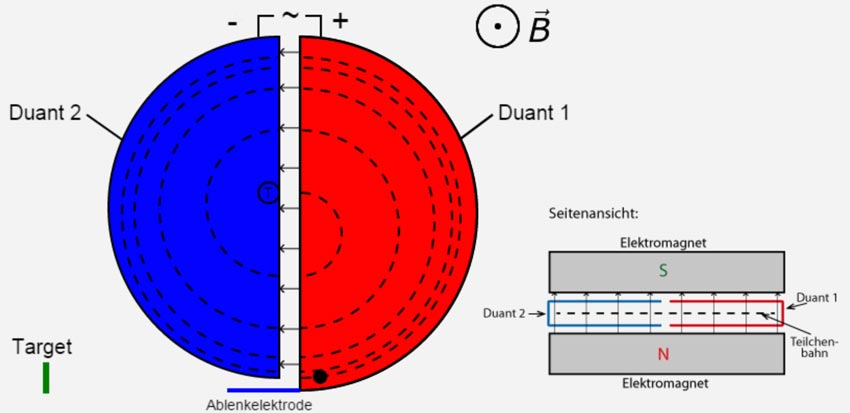
\includegraphics[width=\textwidth]{praes/Aufbau-Zyklotron-de.jpg}
         \footnotemark
        \end{center}
    \end{column}
    \begin{column} {0.5\textwidth}
      \begin{itemize}
        \item<1-> Zweck: Teilchen werden auf hohe Energien beschleunigt
        \item<2-> 2 Duanten (gegen"uber)
        \item<3-> Duanten hohle D-f"ormige K"orper
        \item<4-> Duanten haben einen Abstand zwischeneinander
        \item<5-> Duanten sind von Spulen umgeben
      \end{itemize}
    \end{column}
  \end{columns}
  \footnotetext{http://www.didaktik.physik.uni-muenchen.de/elektronenbahnen/bilder/b-feld/Aufbau-Zyklotron-de.jpg Zugriff: 19.3.2017}
\end{frame}


\begin{frame}
\frametitle{Andere Teilchenbeschleuniger}
\begin{columns}
  \begin{column}{0.33\textwidth}<1->
    \begin{block}{Linearbeschleuniger}
      \begin{itemize}
        \item Gradlinige Beschleunigung
        \item Beschleunigungs-kondensatoren stehen hintereinander
        \item Vorteil: Keine Startgeschwindigkeit notwendig
        \item Nachteil: Nur kurze Beschleunigung m"oglich
      \end{itemize}
    \end{block}
  \end{column}
  \begin{column}{0.33\textwidth}<2->
    \begin{block}{Zyklotron}
      \begin{itemize}
        \item Kreisf"ormige Beschleunigung
        \item konstantes Magnetfeld
        \item konstante Frequenz
        \item Vorteil: Relativ einfache Konstruktion
        \item Nachteil: Maximalgeschwindigkeit
      \end{itemize}
    \end{block}
  \end{column}
  \begin{column}{0.33\textwidth}<3->
    \begin{block}{Synchrotron}
      \begin{itemize}
        \item Kreisf"ormige Beschleunigung
        \item Teilchen laufen in R"ohren
        \item dynamisches Magnetfeld
        \item dynamische Frequenz
        \item Vorteil: Es sind extrem gro"se Geschwindigkeiten m"oglich
        \item Nachteil: Sehr komplexer Aufbau
      \end{itemize}
    \end{block}
  \end{column}
\end{columns}
\end{frame}


\begin{frame}
\frametitle{Wie funktioniert ein Zyklotron ?}
  \begin{columns}[onlytextwidth,t]
    \begin{column} {0.5\textwidth}
      \begin{center}
         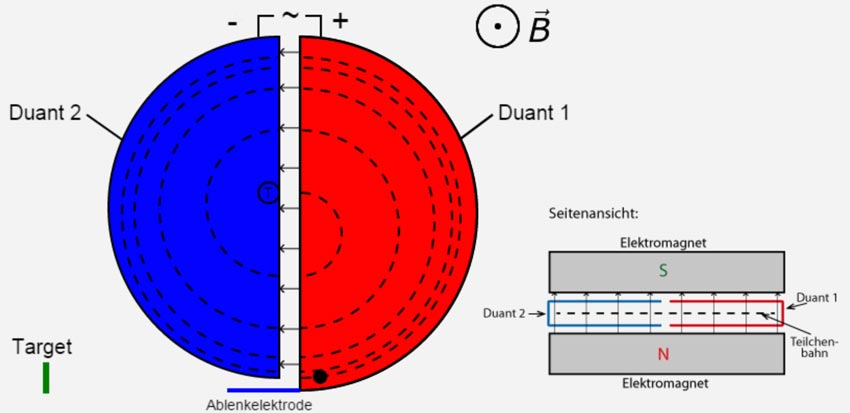
\includegraphics[width=\textwidth]{praes/Aufbau-Zyklotron-de.jpg}
         \footnotemark
        \end{center}
    \end{column}
    \begin{column} {0.5\textwidth}
      \begin{itemize}
        \item<1-> An den Duanten liegt Wechselstrom
        \begin{itemize}
          \item<2-> Volatiles elektrisches Feld zwischen Duanten
          \item<3-> Kein Feld in den Duanten
        \end{itemize}
        \item<4-> Elektrisches Feld kann geladene Teilchen beschleunigen
        \item<5-> Konstanter Strom an den Spulen
        \item<6-> Magnetisches Feld durchsetzt Duanten
        \item<7-> $F_l$ wirkt als $F_z$
      \end{itemize}
    \end{column}
  \end{columns}
  \footnotetext{http://www.didaktik.physik.uni-muenchen.de/elektronenbahnen/bilder/b-feld/Aufbau-Zyklotron-de.jpg Zugriff: 19.3.2017}
\end{frame}


\begin{frame}
\frametitle{Besonderheiten des Zyklotrons}
  \begin{block} {Konstante Umlaufzeit (klassische Vorstellung)}
    Beweis: \\
    \begin{eqnarray}
      F_L       && = F_Z ~~~~ \footnotemark  \\
      Q * v * B     && = \frac{m * v^2}{r} \\
      r     && = \frac{m * v}{Q * B}  ~ | ~ v = \frac{2\pi r}{T} \\
      r     && = \frac{m * 2 * \pi * r}{Q * B * T} \\
      T     && = \frac{m * 2 * \pi }{Q * B} 
    \end{eqnarray}
    \begin{itemize}
      \item T konstant $\rightarrow$ f l"asst sich auf T anpassen
      \item Partikel lassen unendlich lange beschleunigen.
    \end{itemize}
  \end{block}
  \footnotetext{vergleiche Das Gro"se Tafelwerk interaktiv Seite 93}
\end{frame}


\begin{frame}
\frametitle{Relativistische Mechanik im Zyklotron}
  \begin{columns}
    \begin{column}{0.33\textwidth}<1->
      \begin{block}{Zeitdilatation:}
        \begin{itemize}
          \item Die Zeit in bewegten Inertialsystemen vergeht langsamer
          \item F"ur die Simulation unwichtig:
          \begin{itemize}
            \item Zeit aus der Sicht des Teilchens wird nicht gemessen
            \item Wichtig f"ur Zerfallsprozesse
          \end{itemize}
        \end{itemize}
      \end{block}
    \end{column}
    \begin{column}{0.33\textwidth}<2->
      \begin{block}{L"angenkontraktion}
        \begin{itemize}
          \item L"ange in bewegten Inertialsystem ist kleiner
          \item F"ur diese Simulation unwichtig
          \begin{itemize}
            \item Die Breite des Teilchens wird im Modell nicht ber"ucksichtigt
            \item Es wird nicht gemessen welche Strecke das Teilchen zur"ucklegt
          \end{itemize}
        \end{itemize}
      \end{block}
    \end{column}
    \begin{column}{0.33\textwidth}<3->
      \begin{block}{Massenzunahme}
        \begin{itemize}
          \item Bewegte Massen sind schwerer als Ruhemassen
          \item Relevant f"ur die Simulation
          \begin{itemize}
            \item Masse ist wichtig f"ur die Beschleunigung
            \item Masse ver"andert sich, w"ahrend Partikel im Kondensator ist
            \item Geschwindigkeit im Kondensator ist:
              \begin{eqnarray}
                v(t)=\frac{a * t + v_0}{\sqrt{1 + \frac{a * t + v_0}{c}^2}}~~~~\footnotemark\\
                a = \frac{U * Q}{d * m_0}
              \end{eqnarray}
          \end{itemize}
        \end{itemize}
      \end{block}
    \end{column}
  \end{columns}
  \footnotetext{schriftliche Arbeit, Seite 11}
\end{frame}

\begin{frame}
  \frametitle{Das Zyklotron kommt aus dem Takt}
  \begin{enumerate}
    \item <1-> Geschwindigkeit des Teilchens steigt
    \item <2-> Masse steigt
    \item <3-> Umlaufzeit steigt $ T = \frac{m * 2 * \pi }{Q * B} $
    \item <4-> Frequenz und Umlaufzeit stimmen nicht "uberein
    \item <5-> Geschwindigkeit steigt weiter aber langsamer
    \item <6-> positiver und negativer Beschleunigungsanteil gleicht sich
    \item <7-> keine Beschleunigung
  \end{enumerate}
\end{frame}

\begin{frame}
\frametitle{Verwendetes Modell}
\begin{columns}
\begin{column}{0.5\textwidth}
  \uncover<1->{\begin{block}{Teilchen, Felder, Bezugssysteme}
    \begin{itemize}
      \item Teilchen werden als Punkte betrachtet
      \item Felder sind perfekt
      \item Zyklotrone sind Inertialsysteme
    \end{itemize}
  \end{block}}
  \uncover<2->{\begin{block}{Geschwindigkeit (relativistisch)}
    \begin{eqnarray}
      v(t)=\frac{a * t + v_0}{\sqrt{1 + \frac{a * t + v_0}{c}^2}}\\
      a = \frac{U * Q}{d * m_0}
    \end{eqnarray}
    (Ansatz: $\dot{p} = f$ ist n"otig, um Zeit zu verfolgen)
  \end{block}}
\end{column}
\begin{column}{0.5\textwidth}
  \uncover<3->{\begin{block}{Strecke (relativistisch)}
    $s(t)  = \left(\frac{c^2}{a}\right) * \left(\sqrt{1 + \left(\frac{a*t + v_0}{c}\right)^2} - \sqrt{1 + \left(\frac{v_0}{c}\right)^2}\right)$
    (Ansatz: $s = \int{v}$)
  \end{block}}
   \uncover<4->{\begin{block}{weitere Zusammenh"ange}
    F"ur Radius, Umlaufzeit etc. werden klassische Zusammenh"ange mit variabler Masse
    verwendet.
  \end{block}}
\end{column}
\end{columns}
\end{frame}
   

\section{Herausforderung des Projektes}
\frame{\tableofcontents[currentsection]}
\begin{frame}
\begin{block}{Anforderungen}
\textbf{Geschwindigkeit und Genauigkeit}
\end{block}
\end{frame}


\begin{frame}
\frametitle{Geschwindigkeit - Speicher }
\begin{columns}
  \begin{column}{0.5\textwidth}<1->
    \begin{block}{Heap oder Stack}
      \begin{itemize}
        \item  Stack ist geschwindigkeitsoptimiert
        \item  Heapallokation ist teuer und blockend (Syscall)
        \item  Stackallokation sind schneller
        \item  Berechnungen sollen auf dem Stack alloziert werden
      \end{itemize}
    \end{block}
  \end{column}
  \begin{column}{0.5\textwidth}<2->
    \begin{block}{Garbage Collection und Reference Counting}
      \begin{itemize}
        \item  GC unterbricht Programmfluss
        \item  GC pr"uft alle Referenzen
        \item  GC verringert Anzahl der Syscalls
        \begin{itemize}
          \item wird durch Vorallokation in Containern obsolet
        \end{itemize}
        \item RC kostet wenig Rechenzeit ist aber langsamer als manuelles Speichermanagement
      \end{itemize}
    \end{block}
  \end{column}
\end{columns}
\; \; \;
\uncover<3->{
C++ wird als Programmiersprache gew"ahlt, weil sie Kontrolle "uber Heap und Stack gibt}
\end{frame}


\begin{frame}
\frametitle{Geschwindigkeit - Parallele Programmierung}
\begin{itemize}
  \item <1-> Moore's Law
  \item <2-> Also haben CPUs mehr Kerne
  \item <3-> Nebenl"aufige Welt
  \item <4-> Probleme werden nebenl"aufig betrachtet und parallel ausgef"uhrt
  \item <5-> 2 Grundprinzipien (shared Memory);
  \begin{itemize}
    \item <6-> Prinzip: Leichtgewichtprozess oder Thread
    \item <7-> Prinzip: Mutex
  \end{itemize}
\end{itemize}
\end{frame}


\begin{frame}
\frametitle{Genauigkeit - Flie"skommagenauigkeitsproblem }
\begin{itemize}
  \item Floats haben begrenzte L"ange
  \item Zahlen mit begrenzter L"ange verlieren Informationen
  \item kleinster Abstand zwischen 2 Floats: ca. $2.22 * 10 ^{-16}$ \footnote{https://doc.rust-lang.org/std/f64/constant.EPSILON.html letzter Zugriff: 8. Juni 2017}
  \item Elementarladung: $1.609 * 10 ^ {-19}$
\end{itemize}
\begin{columns}
  \begin{column}{0.5\textwidth} 
    \uncover<2->{
    \begin{block}{1. L"osung: Erh"ohung der Zahlenl"ange}
      \begin{itemize}
        \item Integers werden verl"angert (Vector von Digits)
        \item Darstellung von $Q$ als Bruch zweier Integers
        \item Alternativ: Flie"skommazahlen werden verl"angert
        \item Vorteil: Extrem genau
        \item Nachteil: Aufwendig (rechenintensiv und schwierig)
      \end{itemize}
    \end{block}}
  \end{column}
  \begin{column}{0.5\textwidth}
    \uncover<3->{
    \begin{block}{2. L"osung: Wissenschaftliche Darstellung}
      \begin{itemize}
        \item Zahlen werden als $a * 10 ^n$ dargestellt
        \item Nachteil: Problem wird nur verschoben
        \itemize{\item Wird genau genug}
        \item Vorteil: Nicht rechenintensiv
        \item Vorteil: Einfach zu implementieren
      \end{itemize}
    \end{block}}
  \end{column}
\end{columns}
\end{frame}



\section{Wie ist die Simulation aufgebaut ?}
\frame{\tableofcontents[currentsection]}


\begin{frame}
\frametitle{Aufbau des Programms}
\begin{block}{Programmaufbau (vereinfacht)}
\begin{center}
  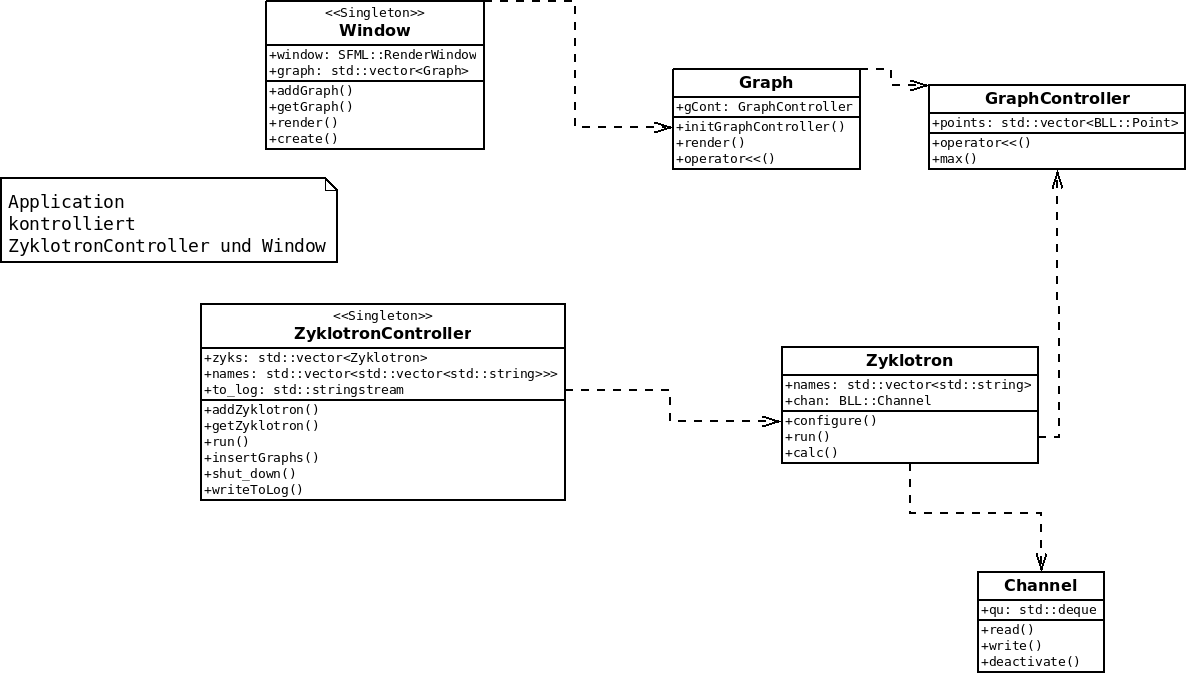
\includegraphics[width=\textwidth]{praes/ProgrammAufbauVereinfacht.png}
\end{center}
\end{block}
\end{frame}

\begin{frame}[fragile]
\frametitle{Implementierungsbesonderheiten}
\begin{block}{Channel}
\begin{columns}
  \begin{column}{0.5\textwidth}<1->
    \begin{lstlisting}{}
      T read() {
         boost::mutex::scoped_lock lock(writemutex);
 
          if (!active) {
              return T{};
          }
 
          while (size == 0) {
              read_cond.wait(lock);
          }
 
          T ret{qu.front()};
          qu.pop_front();
 
          --size;
          read_cond.notify_all();
          return ret;
      }
    \end{lstlisting}
  \end{column}
  \begin{column}{0.5\textwidth}<2->
   \begin{lstlisting}{}
      T write() {
          boost::mutex::scoped_lock 
                lock(writemutex);
 
          if (!active) {
              return T{};
          }
 
          while (size > capacity) {
             read_cond.wait(lock);
          }
 
          qu.push_back(content);

          ++size;
          read_cond.notify_all();         
      }
   \end{lstlisting}
  \end{column}
\end{columns}
\end{block}
\end{frame}


\begin{frame}[fragile]
\frametitle{Implementierungsbesonderheiten}
\begin{block}{StdGraphController}
  \begin{lstlisting}{}
  void StdGraphController::operator<<(BLL::Point p) {
      boost::mutex::scoped_lock{mtx};
      if (points->size() > 1000) {
          auto &points = *this->points;
          std::vector<BLL::Point> *tp = new std::vector<BLL::Point>(500);
          for (int i = 0; i < 500; i++) {
              tp->at(i) = points.at(2 * i);
          }
          auto *op = this->points;
          this->points = tp;
          delete op;
          pointsToFilter *= 2;
          pointsFiltered = 1;
      }
      if (pointsFiltered >= pointsToFilter) {
          (points)->push_back(p);
          pointsFiltered = 1;
      } else {
          pointsFiltered++;
      }
  }
  \end{lstlisting}
\end{block}
\end{frame}



\begin{frame}[fragile]
\frametitle{Implementierungsbesonderheiten}
\begin{block}{Berechnungsschleife}
  \begin{lstlisting}{}
  ZyklotronParts::ZykSet it;
  it.v = this->v0;
  it.time = Double(0, 0);
  const Double a{a0};
  const Double one{1, 0};
  while (running && it.r < r_max) {
      ZyklotronParts::ZykSet res;

      Double c{Double::c()};
      auto &v0 = it.v;

  \end{lstlisting}
  einige Berechnungen auf res
  \begin{lstlisting}{}
    it = res;

    if (!chan)
        return;

    chan->write(std::move(res));
    boost::this_thread::interruption_point();
  }
  to_log = it;
  running = false;
  \end{lstlisting}
\end{block}
\end{frame}


\section{Livedemo}

\frame{\tableofcontents[currentsection]}

\begin{frame}
\frametitle{Literatur}
\begin{itemize}

\item Breymann, Ulrich (2014): Der C++ Programmierer. Hanser, 3.Auflage
\item SFML-Dokumentation: https://www.sfml-dev.org/learn.php, letzter Zugriff: 17.1.2017
\item Boost-Dokumentation: http://www.boost.org/doc/ letzter, Zugriff: 21.2.2017
\item http://en.cppreference.com/w/ letzter Zugriff: 21.12.2016
\item Dr. Bolz/Grehn/Krause/Kr"uger/Dr. Schmidt/Dr. Schwarze (1998): Metzler Physik. Westermann Schroedel Diesterweg
\item Prof. Dr. Erbrecht/Felsch/Dr. K"onig/Dr. Kricke/Martin/Pfeil/Dr. Winter/W"orstenfeld (2014): Das Gro"se Tafelwerk interaktiv. Cornelson-Verlag: 1. Auflage
\item http://schule.mallinckrodt-gymnasium.de/physik/formel.pdf, letzter Zugriff: 19.3.2018
\item Erlenk"otter, Helmut (2003): C Programmieren von Anfang. Rowolt Taschenbuch Verlag, 21. Auflage
\item Meine schriftliche Arbeit
\end{itemize}

\end{frame}

\end{document}

